\section{Zusammensetzung des Ursprungsdatensatzes} \label{sec:Meth Datensatz}
\Gls{ML} benötigt Daten, um aus diesen allgemeingültigen Informationen über eine Aufgabe zu extrahieren. Da die Vorauswahl der Modelle (\autoref{sec:Meth Nutzwert}) deutlich macht, dass Ansätze des überwachten Lernens verfolgt werden, wird auch ein \gls{Labelvektor} benötigt. Wie Ereignisse gelabelt und verifiziert werden, ist in \autoref{sec:Meth Labeling} erläutert. In diesem Abschnitt wird erläutert, wie sich der Ursprungsdatensatz, aus dem später der Trainingsdatensatz und der Testdatensatz hervorgehen, zusammensetzt. Dargestellt wird, wie die Mengenverhältnisse von Kontrollgangereignissen, Kampfereignissen und Normalverhalten sind, bevor die Datenmenge in Bezug auf die Erfolgsaussichten diskutiert wird. 

\subsection{Heraussuchen der Ereignisse}
Wie in \autoref{sec:Meth Labeling} erwähnt, steht für die Verifizierung ein Datensatz mit Ereignissen zur Verfügung. Dieser beinhaltet Ereignisse von allen drei Verhaltensweisen. Die Tabelle \ref{tab:bspUnvDataSet} zeigt den Aufbau dieses Datensatzes exemplarisch. 


\begin{table}[ht]
    \centering
    \caption{Beispielhafter Auszug aus dem Ereignisdatensatz vor der Verifikation.}
    \begin{tabular}{|c|c|c|c|}
        \hline
        Startzeit & Endzeit & KameraID & Label\\
        \hline
        05.05.2021 13:57:00 & 05.05.2021 13:59:00 & 3       & Kampf\\
        \hline
        11.05.2021 06:13:21 & 11.05.2021 06:14:51 & 5       & Kontrollgang\\
        \hline
        \vdots              & \vdots              & \vdots  & \vdots\\
        \hline
        13.06.2021 19:00:03 & 13.06.2021 19:04:17 & 5       & Normalverhalten\\
        \hline
    \end{tabular}
    \label{tab:bspUnvDataSet}
\end{table}

Die Videos wurden angesehen und wenn ein Kampf festzustellen war, wurden über die Laufdauer des Videos die Uhrzeiten geschätzt, zu denen der Kampf stattgefunden hat. Bei einer Untersuchung hat sich herausgestellt, dass die Schätzungen nur grob sind, die Zeitpunktangaben sind ungefähr auf einen Zeitraum von 10 Minuten eingegrenzt. Die Zeitpunkte der Kontrollgänge wurden während der Mastdurchläufe aufgezeichnet. Beim Betreten und Verlassen des Stalls des Tierhalters wurden die Zeitstempel tabellarisch erfasst. Diese sind relativ genau. Die Zeitpunkte des Normalverhaltens wurden zufällig generiert. Da das, was in dieser Arbeit als Normalverhalten deklariert ist, den Großteil der Zeit ausmacht, war zu vermuten, dass mit diesem Vorgehen relativ zuverlässig Normalverhalten markiert wird. Da bei der Generierung der Zeitpunkte die Verifizierung bereits geplant war, war bekannt, dass die zufälligen Zeitpunkte überprüft werden. Die Zeitpunkte des Normalverhaltens wurden Gleichverteilt über den gesamten Mastdurchlauf generiert.\par

Die herausgesuchten Ereignisse entstammen alle dem ersten Mastdurchlauf. Da die manuelle Suche nach Kämpfen sehr zeitintensiv ist, war es im Rahmen dieser Arbeit nicht möglich, weitere Kämpfe herauszusuchen. Die vorhandenen Kämpfe entstammen alle dem ersten Mastdurchlauf und nur aus den Stallbereichen, welche von den Kameras mit den IDs 3 und 5 abgedeckt wurden. Aus diesem Grund wurde sich im Aufbau des Modells auf diesen Mastdurchlauf und die Stallbereiche konzentriert, die von den Kameras Nummer 3 und 5 abgedeckt sind. Der erste Mastdurchlauf ging vom 17.03.2021 bis zum 16.06.2021, wobei die Aufzeichnungen erst am 23.03.2021 begannen. Die Zusammensetzung des Datensatzes dieser herausgesuchten Ereignisse ist in der Tabelle \ref{tab:DataSetUnVeri} zu sehen.\par


\begin{table}[ht]
    \centering
    \caption{Zusammensetzung des Datensatzes der unverifizierten Ereignisse.}
    \begin{tabular}{|l|r|r|}
    \hline
        Verhaltensweise & Anzahl & Anteil \\
    \hline
        Normalverhalten & 160 & 30 \%\\
        Kontrollgang & 159 & 30 \%\\
        Kampf & 216 & 40 \%\\
    \hline
    \hline
        Gesamt & 535 & 100 \%\\
    \hline
    \end{tabular}
    \label{tab:DataSetUnVeri}
\end{table}


\subsection{Verifizierung der Ereignisse und Analysen}
Mittels des Programms zu Verifizierung der Ereignisse lässt sich ein Datensatz erzeugen, in dem die Ereignisse zeitlich möglichst exakt eingegrenzt sind. Auch wird bekannt, welche Ereignisse sich nicht verifizieren lassen, weil sie entweder nicht gefunden wurden, oder weil keine Daten vorhanden sind. Dabei ist aufgefallen, dass vor dem 14.04.2021 die Aufzeichnung stark fehlerhaft verlief. Videostreams sind nicht, oder nur unvollständig vorhanden und die Detektionsdatensätze weisen zeitliche Lücken auf. Somit sind alle Ereignisse vor dem 14.04.2021 nicht verifizierbar. \par

Bei der Verifizierung der Kontrollgänge fiel auf, dass sich diese oft in mehrere Phasen aufteilen. Neben den charakteristischen Merkmalen, die in \autoref{sec:Meth DefAufgabe} beschrieben sind, kehrt dazwischen immer wieder Normalverhalten ein. Bezogen auf den Datensatz bedeutet dies, dass aus einem Kontrollgangereignis sich oft mehrere Phasen extrahieren lassen. Die Tabelle \ref{tab:DataSetVeri} zeigt die Zusammensetzung des Datensatzes nach der Verifizierung, sowie die Veränderung zum Datensatz in \autoref{tab:DataSetUnVeri}. 

\begin{table}[ht]
    \centering
    \caption{Zusammensetzung des Datensatzes nach der Verifizierung.}
    \begin{tabular}{|l|r|r|r|}
    \hline
        Verhaltensweise & Anzahl & Anteil & Veränderung\\
    \hline
        Normalverhalten & 103 & 21 \% & -36 \%\\
        Kontrollgang & 188 & 39 \% & +18 \%\\
        Kampf & 196 & 40 \% & -9 \%\\
    \hline
    \hline
        Gesamt & 487 & 100 \% & -9 \% \\
    \hline
    \end{tabular}
    \label{tab:DataSetVeri}
\end{table}

Insgesamt sorgt die Verifizierung dafür, dass die Gesamtanzahl der Ereignisse schrumpft. Durch die Aufteilung der Phasen der Kontrollgänge ist ein Zuwachs der Kontrollgangereignisse festzustellen. Von Interesse ist auch die Dauer der Ereignisse. Gerade die Kontrollgänge und Kämpfe zeigen eine zeitliche Begrenzung, während das Normalverhalten eher als der Normalzustand betrachtet wird, der von einem Kampf oder Kontrollgang unterbrochen wird. Dadurch besitzt Normalverhalten keinen klar definierten Start- und Endpunkt. Bei der Verifizierung sind Start- und Endpunkt vom Normalverhalten also eher so zu interpretieren, dass sichergestellt wird, dass sich in diesem Zeitraum kein Kampf und kein Kontrollgang abspielt. In der Abbildung \ref{fig:EreignisDauer} sind die unterschiedlichen Längen der Ereignisse in Histogrammen dargestellt.

\begin{figure}[htbp]
    \centering
    \begin{subfigure}{.5\textwidth}
        \centering
        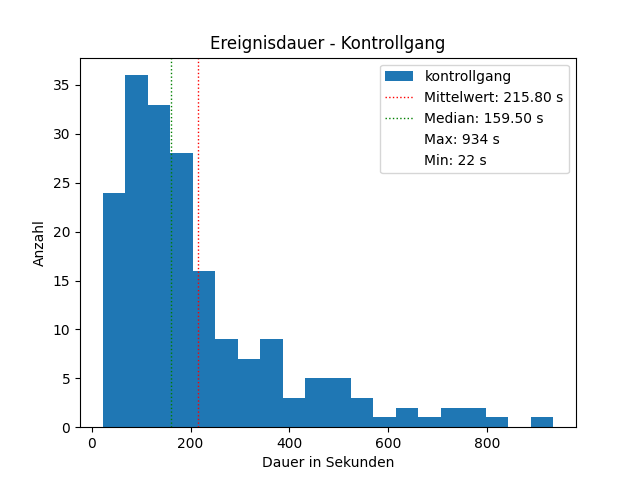
\includegraphics[width=1.1\linewidth]{img//Ereignisdauer/Auswertung Ereignisdauer kontrollgang.png}
        \caption{Kontrollgang}
        \label{fig:DauerKontroll}
    \end{subfigure}%
    \begin{subfigure}{.5\textwidth}
        \centering
        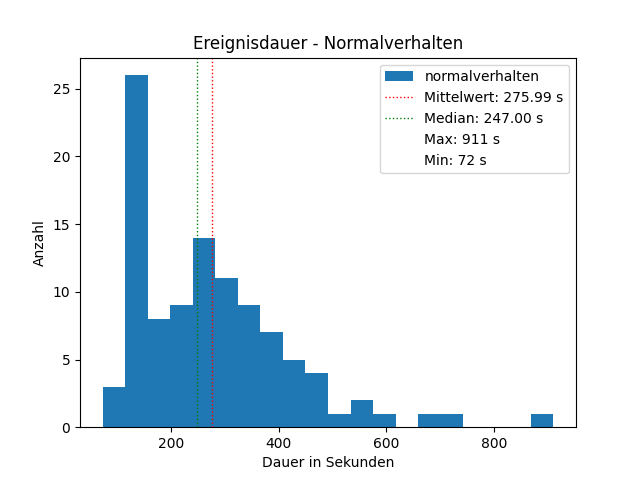
\includegraphics[width=1.1\linewidth]{img//Ereignisdauer/Auswertung Ereignisdauer normalverhalten.png}
        \caption{Normalverhalten}
        \label{fig:DauerKampf}
    \end{subfigure}
    \begin{subfigure}{.6\textwidth}
        \centering
        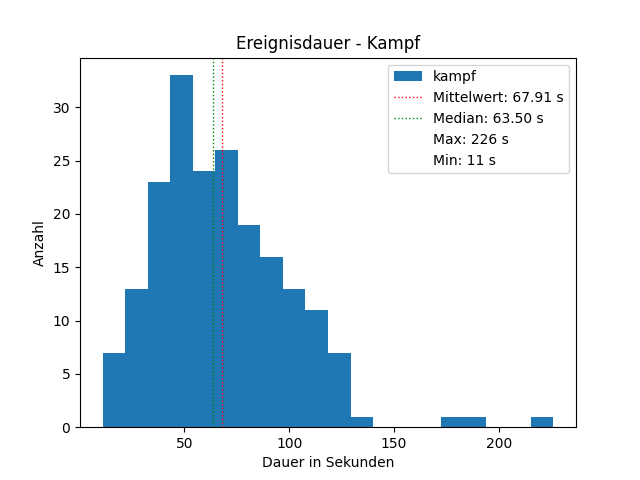
\includegraphics[width=1\linewidth]{img//Ereignisdauer/Auswertung Ereignisdauer kampf.png}
        \caption{Kampf}
        \label{fig:DauerNormal}
    \end{subfigure}
    \caption[Histogramme der zeitlichen Längen der Ereignisse im verifizierten Datensatz.]{Histogramme der zeitlichen Längen der Ereignisse im verifizierten Datensatz. (a) zeigt die Dauer der Kontrollgänge. In (b) sind die Längen des Normalverhaltens zu sehen. (c) zeigt die Kampfereignisse. Es sind jeweils der Mittelwert und der Median eingezeichnet. In der Legende sind Minmal- und Maximalwerte angegeben.}
    \label{fig:EreignisDauer}
\end{figure}

\subsection{Erstellung des Ursprungsdatensatzes}
In \autoref{fig:EreignisDauer} fällt auf, dass die unterschiedlichen Ereignisse sehr unterschiedlich lang seien können. Kontrollgänge sind i.d.R deutlich länger als Kämpfe. Aber auch innerhalb einer Verhaltensweise kann die Länge deutlich variieren. Es ist zu sehen, dass die Kämpfe im Schnitt am kürzesten sind. Diese dauern meistens nur ungefähr eine Minute. Auch das kürzeste Ereignis ist ein Kampf mit 11 Sekunden. Da die ausgewählten Modelle die Zeitreihen der Ereignisse in Form von komprimierten Features erhalten sollen, macht die Varianz in den Längen die Vergleichbarkeit kompliziert. Bezogen auf die Anwendung des Moduls zur Verhaltensklassifikation ist das herausfordernd, da das Modul nicht weiß, wie lang das aktuell abgetastete Ereignis ist und wie viele Zeitschritte es zur Erkennung von diesem komprimieren muss. \par

Um dieses Problem zu lösen, werden die Ereignisse in gleich große Abschnitte zerteilt. Ein Kontrollgangereignis, das 6 Minuten geht, wird bspw. in 6 Abschnitte von jeweils einer Minute Länge geteilt. Das Gleiche geschieht mit allen Ereignissen, sodass ein Datensatz entsteht, in dem alle Ereignisse die gleiche Länge haben. Für die Anwendung ist das vorteilhaft, da das Modul somit feste Intervalle auswertet. Dadurch wird keine Abschätzung der Ereignisdauer benötigt. \par

Es ist zu bestimmen, welche Intervalllänge für das Modul und die Aufgabe geeignet ist. Dazu sind die Faktoren zu betrachten, die damit in einem Zusammenhang stehen. Um eine konstante lückenlose Abtastung des Stallgeschehens zu erreichen, darf das Intervall maximal so lang sein wie die Laufzeit des Moduls. Wünschenswerter ist jedoch, dass sich die Intervalle bei der Abtastung überlappen. Ist das nicht der Fall, kann es passieren, dass ein Ereignis so zerteilt wird, dass die charakteristischen Merkmale in der Kompression nicht mehr deutlich werden. Bei einer Überlappung der Intervalle wird die Gefahr reduziert, dass ein Ereignis nicht erkannt wird. Von der Laufzeit des Moduls ist zu diesem Zeitpunkt nur die Laufzeit des Assoziationsmoduls abschätzbar, wie in \autoref{sec:Ergebnisse MOT} dargestellt wird. Aus diesem Grund ist genügend Puffer wichtig, um im Nachhinein keine Komplikationen durch die Laufzeit des Moduls zu erhalten. Der Puffer darf jedoch nicht zu groß sein. Ist der Intervall deutlich größer als das Ereignis selbst, verwässern die charakteristischen Merkmale bei der Komprimierung. Ist der Intervall zu klein, werden die charakteristischen Merkmale nicht deutlich in den komprimierten Features. Auch die Echtzeitfähigkeit muss beachtet werden. Die Intervalle dürfen nicht länger sein, als ein Ereignis dauert. Sonst ist keine Einflussnahme auf das Ereignis möglich.\par

Die optimale Länge des Intervalls ist schwer zu bestimmen. Über die Laufzeiten in der Abbildung \ref{fig:EreignisDauer} lässt sich jedoch eingrenzen, mit welcher Intervalllänge ein funktionierendes Modul zu erwarten ist. Die minimale Ereignisdauer eines Kampfes und eines Kontrollgangs lässt sich als untere Grenze für das Intervall annehmen. Es kann sein, dass die charakteristischen Merkmale bereits mit einer kürzeren Dauer eindeutig festzustellen sind. Mit der Annahme der minimalen Ereignisdauer wird jedoch sichergestellt, dass die Merkmale erfasst werden. Diese ist für die Kontrollgänge, mit 22 Sekunden, länger als bei Kämpfen. Um einen Kontrollgang eindeutig zu erfassen, wird angenommen, dass das Intervall mindestens 22 Sekunden umfassen muss. \par

Aus dem Mittelwert und Median der Kampfdauer lässt sich eine Eingrenzung der maximalen Intervalldauer ableiten. Der Mittelwert liegt bei 68 Sekunden und der Median bei 64 Sekunden. Um die Erfassung der charakteristischen Merkmale von Kämpfen nicht zu verwässern, ist es sinnvoll, unterhalb des Medians zu bleiben. \par

Dass in der Anwendung der Start eines Ereignisses exakt auf den Anfang eines Intervalls fällt, ist unwahrscheinlich. Damit dennoch möglichst frühzeitig ein Ereignis erkannt werden kann,  ergibt es Sinn, einen gewissen Grad der Verwässerung zu erlauben, bei dem die charakteristischen Merkmale weiterhin sichtbar genug bleiben. Der Grad wird auf 75 \% geschätzt, sodass dieser Anteil eines Intervalls die charakteristischen Merkmale beinhalten muss, damit dieses erkannt werden kann. Bezogen auf die untere Grenze von 22 Sekunden bedeutet dies, dass das Intervall maximal 29 Sekunden lang sein darf, damit auch die kürzesten Kontrollgänge noch frühzeitig detektiert werden. \par

Um genügend Puffer für die Laufzeit des Moduls einzuplanen, wird das Intervall auf eine Länge von 40 Sekunden gesetzt. Für einen größeren Puffer wird in Kauf genommen, dass die kürzesten Ereignisse nicht erkannt werden können. Ereignisse, die kürzer als \(40 s \cdot 75 \% = 30 s\) sind, werden so nicht registriert. Die Tabelle \ref{tab:DataNachIntervall} zeigt, wie sich das auf die Menge der Ereignisse auswirkt, die genutzt werden können.\par

\begin{table}[ht]
    \centering
    \caption{Zusammensetzung des Datensatzes nach Festlegen des Intervalls.}
    \begin{tabular}{|l|r|r|r|}
    \hline
        Verhaltensweise & Anzahl & Anteil & Veränderung\\
    \hline
        Normalverhalten & 103 & 22 \% & -0 \%\\
        Kontrollgang & 186 & 40 \% & +1 \%\\
        Kampf & 175 & 39 \% & -11 \%\\
    \hline
    \hline
        Gesamt & 470 & 100 \% & -5 \% \\
    \hline
    \end{tabular}
    \label{tab:DataNachIntervall}
\end{table}

Da nun das Intervall feststeht, können die Ereignisse auf feste Längen aufgeteilt werden. Um \gls{Leakage} zu vermeiden, geschieht dies ohne Überlappung. Damit das Modell lernen kann, ein Ereignis zu erkennen, das nicht die vollen 40 Sekunden umfasst, werden Proben benötigt, in denen das Ereignis in einer Länge von 30 bis 40 Sekunden stattfindet. Dazu werden die Startzeitpunkte und die Endzeitpunkte der Ereignisse auf die nächsten vollen 10 Sekunden gerundet. Die Startzeitpunkte werden abgerundet und die Endzeitpunkte werden aufgerundet. Der Startzeitpunkt \(13:00:57\) würde dementsprechend auf \(13:00:50\) vorgezogen werden und der Endzeitpunkt \(13:02:17\) verschiebt sich nach hinten auf \(13:02:20\). \par

In der Tabelle \ref{tab:DataNachIntervall} ist zu sehen, dass die Gesamtanzahl der Ereignisse dadurch um 5 \% reduziert wird. Am negativsten wirkt sich das Intervall auf die Kampfereignisse aus. Diese werden um 11 \% verringert. Da die Kampfereignisse von großem Interesse sind, ist dieser Datenverlust beträchtlich. Er wird jedoch in Kauf genommen, da die restlichen Kampfereignisse somit sicher die charakteristischen Merkmale beinhalten und das in einer Intensität, mit der das Modul diese sicher erkennen kann, was sich ferner positiv auf die Datenqualität auswirken sollte. \par

Mit diesen Überlegungen können die Ereignisse zerteilt werden. In der Tabelle \ref{tab:DatasetSplit} ist zu sehen, welche Datenmengen sich dadurch ergeben. 

\begin{table}[ht]
    \centering
    \caption{Zusammensetzung des Datensatzes nach der Aufteilung gemäß dem Intervall.}
    \begin{tabular}{|l|r|r|r|}
    \hline
        Verhaltensweise & Anzahl & Anteil \\
    \hline
        Normalverhalten & 683 & 35 \% \\
        Kontrollgang & 969 & 50 \% \\
        Kampf & 290 & 15 \% \\
    \hline
    \hline
        Gesamt & 1942 & 100 \%\\
    \hline
    \end{tabular}
    \label{tab:DatasetSplit}
\end{table}

Bei der Feature-Extraktion und Konstruktion fiel auf, dass die Detektion im Stall erst ab dem 19.04.2021 stabil lief.Die vorherigen Detektionsdatensätze beinhalten viele Einträge, in denen nichts detektiert wurde. Aus den Ereignissen in diesem Zeitraum sind keine Features extrahierbar, weshalb sie nicht für den Aufbau des Modells verwendet werden können. Die Tabelle \ref{tab:DatasetFeatExtr} zeigt die Auswirkungen auf die Datenmenge.

\begin{table}[ht]
    \centering
    \caption{Zusammensetzung des Datensatzes nach der Aufteilung gemäß dem Intervall.}
    \begin{tabular}{|l|r|r|r|}
    \hline
        Verhaltensweise & Anzahl & Anteil & Veränderung\\
    \hline
        Normalverhalten & 572 & 40 \% & -16 \%\\
        Kontrollgang & 868 & 61 \% & -10 \%\\
        Kampf & 220 & 15 \% & -24 \%\\
    \hline
    \hline
        Gesamt & 1660 & 100 \% & -15 \% \\
    \hline
    \end{tabular}
    \label{tab:DatasetFeatExtr}
\end{table}


\subsection{Diskussion der Datenmenge}
Vorteilhaft ist, dass sich durch die Aufteilung gemäß den Intervallen die Anzahl der Proben deutlich erhöht hat. Für \gls{ML} kann die Datenmenge entscheidend sein. Mit 1660 Ereignissen ist die Datenmenge in diesem Kontext relativ klein. Hinzu kommt, dass der Datensatz unbalanciert ist. Der Anteil der Kämpfe ist deutlich niedriger als der Anteil der anderen beiden Verhaltensweisen. Damit war zu rechnen, da die Kontrollgänge und das Normalverhalten im Schnitt deutlich länger sind als Kämpfe, wie in den Histogrammen in \autoref{fig:EreignisDauer} zu sehen ist. Durch die Einteilung in die Intervalle entstehen aus einem Kontrollgang somit mehr Proben, als aus einem Kampfereignis. Um mit dem Datensatz ein Modell zu trainieren, ist es ratsam dieses mittels Undersampling auszubalancieren (\autoref{sec:Datensätze ML}). Dadurch reduziert sich die effektiv nutzbare Datenmenge, wie in Tabelle \ref{tab:DataNachBalance} dargestellt.

\begin{table}[ht]
    \centering
    \caption{Zusammensetzung des Datensatzes nach Festlegen des Intervalls.}
    \begin{tabular}{|l|r|r|r|}
    \hline
        Verhaltensweise & Anzahl & Anteil & Veränderung\\
    \hline
        Normalverhalten & 220 & 33 \% & -62 \%\\
        Kontrollgang & 220 & 33 \% & -75 \%\\
        Kampf & 220 & 33 \% & -0 \%\\
    \hline
    \hline
        Gesamt & 660 & 100 \% & -60 \% \\
    \hline
    \end{tabular}
    \label{tab:DataNachBalance}
\end{table}

Bei dem Aufbau des Modells ist ein großes Risiko für Overfitting vorhanden. Durch die Verifizierung der Ereignisse besteht jedoch die Hoffnung, dass die Qualität der Daten hoch ist. Das erhöht die Chancen für ein funktionierendes Modell. \par

Der Datensatz besitzt einen Bias durch geringe Varianz. Die Daten stammen aus nur einem Mastdurchlauf und damit aus einem sehr begrenzten Zeitraum von zwei Monaten (19.04.2021 bis zum 16.06.2021). Es sind nur die beiden Kameras mit den IDs 3 und 5 ausgewertet worden. Dadurch besteht auch hier ein Bias in Bezug auf den Stallbereich. Diese Voreingenommenheiten können dafür sorgen, dass sich das Modell schlecht auf beliebige Stallbereiche anwenden lässt\par

Zusammenfassend lässt sich sagen, dass die Datenlage unvorteilhaft ist, um ein Modell aufzubauen, das gut generalisieren soll. Die Datenqualität kann dem möglicherweise entgegenwirken. Das Bewusstmachen der Schwächen der Datengrundlage kann dazu genutzt werden, im Featureengineering und in der Modellkonfiguration Gegenmaßnahmen zu ergreifen – gerade in Bezug auf die Vermeidung von Overfitting.